\todo{Prima!}
\section{Methodology}
\label{sec:meth}
The following sections will describe the stages required to examine the suitability of Frog for doing NER on parliamentary items. Firstoff a description of the data is given in section \ref{subsec:data}. The employment of Frog is apparent in section \ref{subsec:frog_emp}. Subsection \ref{subsec:eval_prep} will then eloborate the preparation needed to evaluate Frog on the CoNLL-2002 data set and the set of parliamentary items. Lastly, from subsection \ref{subsec:reclas} can be understood how reclassification of entity types was performed. 

\subsection{Description of the data}\label{subsec:data}

\todo{Dit vind ik toch wel mal. Waarom noem je dit lobby documents? Kijk eens op \url{https://zoek.officielebekendmakingen.nl/zoeken/parlementaire_documenten}, daar komen ze vandaan. Noem die pagina ook. Dit zijn officiele stukken gepubliceerd door het Nederlandse parlement. Zo moet je ze noemen. Dat lobbyisten ze willen gebruiken is een heel ander verhaal. Ook al is het waar.}

\todo{Ik zou ook wat zeggen over de tijdsperiode waarde documenten itkomen, desnoods alleen in de caption van je tabelletje}
The dataset is a set of lobby documents that has been scraped from the web. Lobbying can be defined as the act of attempting to influence decisions made by officials in a government, most often legislators or members of regulatory agencies. Lobby documents are for example: resolutions, chamber inquiries, letters to the government and more. A distribution of different types can be seen in figure \ref{fig:data_dis}. The result of scraping these documents is that certain figures or itemization structures are textualized into words concatenated with itemization numbers, table entry titles or something alike. Nevertheless, Frog's tokenization module will most of the time seperate the tokens correctly.  The documents have been exported as consistent JSON dicts (a sample can be seen in figure \ref{fig:data_form}) with for each document its corresponding meta information such as its ID, source, and type. The content of the item in the figure has been omitted, but that is the dict entry where the complete item can be found. The JSON format can easily be read with Python. For domain reduction purposes, only parliamentary items are included in the data set. These items form the majority of the items and are a mix of all types, except for the news items, in which, undesirably, NE's vary greatly in domain compared to the parliamentary items.

\begin{figure} \label{fig:data_dis}
\centering
\begin{tabular}{l|r}
Type              & Count \\
\hline
Parliamentary item & 131906  \\
News item & 95261 \\
Chamber inquiry & 38804  \\
Voting & 20930 \\
Chamber letter & 19828 \\
Agenda item & 18950  \\
Resolutions & 4792 \\
\end{tabular}
\caption{The distribution of the initial data}
\end{figure}

\begin{figure}
    \centering
    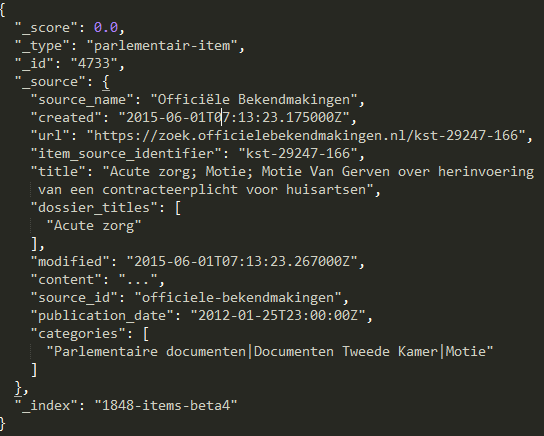
\includegraphics[scale=0.8]{fig/data_format}
    \caption{A sample of a parliamentary item represented as a JSON dict}
    \label{fig:data_form}
\end{figure}

\subsection{Employment of Frog}\label{subsec:frog_emp}
Frog is open-source software that can be modified or redistributed under the GNU General Public License\footnote{\url{http://www.gnu.org/copyleft/gpl.html}}. The results in this paper have been acquired by running Frog through a virtual machine on Windows. All necessary dependencies of Frog, including Frog itself, are provided by the LaMachine software distribution\footnote{\url{https://proycon.github.io/LaMachine/}}. Frog has been launched through Python using the python-frog binding which is also included in the virtual machine.

\subsection{Evaluation preparation}\label{subsec:eval_prep}
Differences in format and annotation guidelines had to be overcome in order to make an evaluation. 
Additionally a golden standard for parliamentary items has been created.
\subsubsection{Format difference}
The CoNLL-2002 data set uses the following format: $$TOKEN\,[whitespace]\,POS\,[whitespace]\,ENTITY$$ Every line contains three elements, each seperated by a whitespace: the token, which is an unprocessed word from a sentence, its corresponding part-of-speech, and the entity tag that belongs to the token. The Folia format, with tab-delimited columns instead of whitespaces looks similar, but comes without additional columns of token information. To release Frog on CoNLL, the test set first has to be reformatted to its original text. This is done by removing the PoS- and entity tags, concatenating the remaining words into their original sentences thereafter.  Frog chunks together multi-word entities and other words that are closely related on the same line in the output. This will make it differ from the CoNLL output, as is why the output is resplitted with python using regular expressions. Superfluous information is removed from each line. The ultimate processed text has the same format as CoNLL, which implies identical line mapping per token.

\subsubsection{Guideline difference}
It needs to be considered that the annotation guidelines for the SoNaR corpus, on which Frog is trained, differ from CoNLL. SoNaR has a wider range of entity types, with addition of EVE for event and PRO for product. These types are annotated in CoNLL as MISC. Therefore these additional types have been mapped to MISC. There is also a guideline difference regarding locational adjectives, such as 'Dutch' or 'European'. CoNLL guidelines\footnote{\url{http://www.cnts.ua.ac.be/conll2003/ner/annotation.txt}} state to annotate such an adjective as MISC, while Frog is trained to assign LOC as type. These LOC outputs of Frog have been reassigned to MISC as well.

\subsubsection{Parliamentary items: golden standard}
\todo{Graag wat meer informatie: bijvoorbeeld hoeveel entities van elk type, hoeveel entities van elke lengte (aantal tokens), etc, En geef wat voorbeelden: bijvoorbeeld de top meeste voorkomende. Maak het wat minder droog op die manier.}
A test set of 35.338 tokens has been constructed as a golden standard to compare Frog-processed parliamentary items to. As basis, Frog output of the tokens used for the golden standard set is formatted the same as CoNLL, keeping PoS as determined by Frog. All entity tags are changed to \textit{O} beforehand to prevent bias in the annotation process. Subsequently, all entity tags have been manually assigned pursuing the CoNLL annotation guidelines. This golden standard is publicly available for download\footnote{$^{soon}$}. 

\subsection{Reclassification of entity types}\label{subsec:reclas}
Reclassification of entity types has been done in two steps. Majority voting is only applicable when the gazetteer step has had no success.
\subsubsection{Gazetteer}
Firstly, all found entities are re-evaluated by search in a gazetteer in the domain of parliamentary items. This gazetteer has been constructed with a combination of automatic extraction of entities with Frog and manual annotation of the correct type. The automatic extraction is performed on the training set of thousand parliamentary items. These parliamentary items have been processed with Frog resulting in a dump that contains the occurrence counts per entity over all items. The dump has then been sorted descendingly, giving annotation priority to the most common entities. The effectiveness of this step is dependent on: 
\begin{enumerate} 
\item The amount of entities manually annoted in the gazetteer
\item The recall performance of Frog 
\item The size of the training set 
\item The relevance of the training set. 
\end{enumerate}
It needs to be acknowledged that entities that do not appear in the gazetteer cannot be reclassified in this step.

\subsubsection{Majority voting}
In the case of unknown words the contextual word relations may indicate a type correctly, however, with multiple occurrences of the same entity throughout a text, context differs from time to time. As a result an unambiguous entity can be tagged correctly as a PER 90\% of the time, but have an incorrect type assigned for the remaining 10\%. This is expected to be resolved using majority voting. In the case where a certain type is dominant over a minority, this minority is reclassified as the dominant type. To retrieve information regarding the dominant types per entity, a train set of thousand parliamentary items has been processed by Frog. The total occurrences of the entity types have been counted over all documents. For each token in the test set that has been assigned an entity tag, majority voting has been applied. Whether an entity type is dominant for that entity is decided based on a threshold value. When the fraction of an entity type over the total amount of entity type counts is larger than the threshold value, the type is considered dominant. The formula for majority voting, as well a the complete reclassification procedure in pseudocode is apparent in algorithm \ref{alg:pseudo}.

\begin{algorithm} \label{alg:pseudo}
    \SetKwInOut{Input}{Input}
    \SetKwInOut{Output}{Output}

    \underline{reclassify} $(frogged\_file, vote\_file, gazetteer\_file)$\;
    \Input{Three files (path) each containing: the output of the Frogged text in folia-XML format, a dict of the counts for each type per entity, a dict of entities and their correct type}
    \Output{CoNLL format with reclassified types}
    treshold $\leftarrow$ 0.7\\
    type\_counts $\leftarrow$ load(vote\_file)\\
    gazetteer $\leftarrow$ load(gazetteer\_file)\\
    \ForEach{line in frogged\_file}{
        token, lemma, pos, chunk, iob+type etc. $\leftarrow$ split(line)\\
        iob $\leftarrow$ split(iob+type-tag)\\
        \If{is\_entity(token)}{
            new\_type $\leftarrow$ lookup(token, gazetteer)\\
            \tcp{if token is in gazetteer, no majority vote needed}
            \eIf{new\_type}{
                line $\leftarrow$ token, pos, iob+new\_type\\
            }{
                new\_type $\leftarrow$ vote\_type(token, type\_counts, treshold)\\
                \If{new\_type}{
                    line $\leftarrow$ token, pos, iob+new\_type\\
                }
            }
            
        }
    }
    
    \underline{vote\_type} $(token, type\_counts, treshold)$\;
    \Input{token of which to decide the type, the type\_counts dictionary, and the treshold to enact on revoting}
    \Output{new type for the token, none returned otherwise}
    new\_type $\leftarrow$ max(type\_counts[token])\\
    confidence\_score $\leftarrow$ max(type\_counts[token]) / total(type\_counts[token])\\
    \If{confidence\_score $\textgreater$ treshold}{
        \Return{new\_type}
    }
        
    \caption{Reclassification of entity types in Frog output using majority voting and a type gazetteer}
\end{algorithm}





